\newpage
\section{Valore assoluto}
\begin{definition}[Valore assoluto]
    Dato $x \in \mathbb{R}$ si dice valore assoluto di x il massimo valore fra x e -x e si indica con $|x|$.
    \begin{equation}
        |x| = max(\{x, -(x)\})
    \end{equation}
\end{definition}
\begin{example}
    Esempi valore assoluto:
    \begin{itemize}
        \item $|5| = max(\{5, -5\}) = 5$
        \item $|-3| = max(\{-3, -(-3)\}) = 3$
    \end{itemize}
\end{example}
\subsection{Proprietà valore assoluto}
\begin{table}[h!]
    \setlength{\tabcolsep}{7pt}
    \renewcommand{\arraystretch}{2}
    \centering
    \begin{tabular}{|c|c|}
        \hline
        (1) $x \leq |x| \: \: \forall \: \: x \in \mathbb{R}$ & (2) $|x| = x$ se $x \geq 0, |x| = -x$ se $x \leq 0$ \\
        (3) $|x| \geq 0 \: \: \forall \: \: x \in \mathbb{R}$ & (4) $|x| = 0 \Longleftrightarrow x = 0$ \\
        (5) $|-x| = |x|$ & (6) $-|x| \leq x \leq |x|$ \\
        (7) $|x| \leq M \Longleftrightarrow -M \leq x \leq M$ con $M \geq 0$ & (8) $|x| \geq M \Longrightarrow x \geq M$ oppure $x \leq -M$ \\ \hline
    \end{tabular}
    \caption{Proprietà valore assoluto}
    \label{tab:prop-valore-assoluto}
\end{table}
\subsubsection{Spiegazioni proprietà}
Se stabiliamo un punto M maggiore del valore assoluto la funzione si troverà compreso fra M e -M. Se invece stabiliamo un punto M minore del valore assoluto la funzione sarà maggiore di M e minore di -M. Spiegazione grafica nell'immagine [\ref{fig:prop-6-7}]
\begin{figure}[h!]
    \centering
    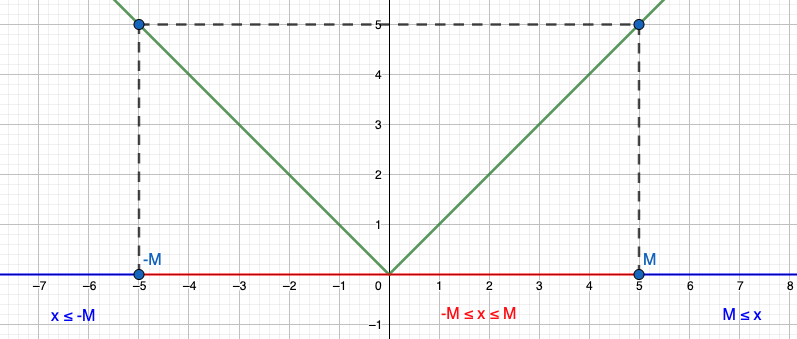
\includegraphics[width=10cm]{es-proprieta-valore-assoluto.png}
    \caption{Spiegazione proprietà 7 e 8}
    \label{fig:prop-6-7}
\end{figure}

\subsection{Disuguaglianza triangolare}
\begin{definition}[Disuguaglianza triangolare]
    Dati due valore $a$ e $b$ tali che $a, b \in \mathbb{R}$ risulta che:
    \begin{equation}
        (1)\:\:\:|a + b| \leq |a| + |b| \hspace{.7cm} (2)\:\:\:||a| + |b|| \leq |a - b| 
    \end{equation}
\end{definition}
\begin{demostration}
    Dimostrazione proprietà (1):\\
    Dati due valori $a$ e $b$ calcoliamo il valore assoluto, che per la proprietà (6) in tabella \ref{tab:prop-valore-assoluto}  possiamo scrivere nella seguente forma:
    \begin{equation}
            -|a| \leq a \leq |a| \hspace{.6cm} -|b| \leq b \leq |b|
    \end{equation}
    Ora facciamo una somma di disuguaglianze fra le forme riportate sopra:
    \begin{equation}
        - |a| - |b| \leq a + b \leq |a| + |b|
    \end{equation}
    Possiamo vedere la prima parte $-|a| - |b|$ come un -M, la parte $a + b$ come una $x$ e l'ultima parte $|a| + |b|$ come M. Utilizzando a questo punto la proprietà (7) in tabella \ref{tab:prop-valore-assoluto}, $|x| \leq M$ quindi:
    \begin{equation}
        |a + b| \leq |a| + |b|
    \end{equation}
\end{demostration}
\begin{observation}
Perché una disuguaglianza triangolare a 3 numeri, $|a + b + c| \leq |a| + |b| + |c|$, vale?\\ \\
Perché se $|a + b + c|$ lo dividiamo in $|(a + b) + c|$ possiamo applicare la propria triangolare su 2 valori considerando $(a+b)$ il primo e $c$ il secondo questo fa si che $|(a + b) + c| \leq |a + b| + |c|$ andando poi a riapplicare la disuguaglianza triangolare questa volta solo su $|a + b|$ vediamo che:
\begin{equation}
    |a + b + c| = |(a + b) + c| \leq |a + b| + |c| \leq |a| + |b| + |c|
\end{equation}
Da qui possiamo dedurre che la disuguaglianza triangolare vale indipendentemente dal numero di valori:
\begin{equation}
    |a_1, a_2, a_3, ..., a_n| \leq |a_1| + |a_2| + |a_3| + .... + |a_n|
\end{equation}
\end{observation}